\chapter{Identificar sustancias}\label{ch:g7:identifying-substances}

En el escenario de un pequeño misterio aparece una nota arrugada,
escrita con rotulador negro, y en tres bolsas distintas se encuentran
tres rotuladores. A simple vista, las tres tintas tienen el mismo negro.
A un químico forense le bastan una tira de papel, un poco de agua y
media hora para decir qué rotulador escribió la nota. Los químicos no
identifican las sustancias por su aspecto, sino por cómo se comportan en
un ensayo elegido para ellas.

\begin{recall}
Una \omterm{def:g6:pure-substances-and-mixtures:species}{especie química} es una clase concreta de sustancia; una \omterm{def:g6:pure-substances-and-mixtures:pure-substance}{sustancia
pura} contiene una sola especie, y una \omterm{def:g6:pure-substances-and-mixtures:mixture}{mezcla}, varias
(\cref{ch:g6:pure-substances-and-mixtures}). Unas sustancias se
\omterm{def:g2:mixing-and-dissolving:dissolve}{disuelven} bien en un \omterm{def:g6:solutions-and-solubility:solute}{disolvente} y otras poco o nada: cada una tiene su
propia \omterm{def:g6:solutions-and-solubility:solubility}{solubilidad} (\cref{ch:g6:solutions-and-solubility}).
\end{recall}

\section{Qué es un ensayo característico}

\begin{definition}[Ensayo característico y reactivo]\label{def:g7:identifying-substances:characteristic-test}
Un \emph{ensayo característico}\index{ensayo caracteristico@ensayo característico} de una
\omterm{def:g6:pure-substances-and-mixtures:species}{especie química} es un experimento sencillo que da un resultado visible
con esa especie, y no con las demás que pueden aparecer en la misma
situación. Utiliza una sustancia elegida para ello, el
\emph{reactivo}\index{reactivo}.
\end{definition}


\begin{method}[Realizar un ensayo característico]\label{met:g7:identifying-substances:run}
\begin{enumerate}
  \item Tomar una pequeña muestra de la sustancia que se quiere ensayar.
  \item Añadir el \omterm{def:g7:identifying-substances:characteristic-test}{reactivo}, o ponerlo en contacto con la muestra, como
        indica el ensayo.
  \item Observar: un cambio de color, una turbidez, una llama, un
        sonido.
  \item Concluir: el ensayo es \emph{positivo} si aparece el resultado
        esperado, y \emph{negativo} si no aparece.
  \item Hacer el mismo ensayo con una muestra que se sabe que no
        contiene la especie (un ensayo en blanco): debe salir negativo;
        si no, el resultado no demuestra nada.
\end{enumerate}
\end{method}

\section{Cuatro ensayos clásicos}

\begin{proposition}[El dióxido de carbono enturbia el agua de cal]\label{prop:g7:identifying-substances:limewater}
El agua de cal es una disolución transparente e incolora. Cuando se hace
burbujear dióxido de carbono a través de ella, se vuelve lechosa, de un
blanco turbio. El \omterm{def:g4:air-a-mixture-of-gases:air}{aire} espirado con una pajita enturbia el agua de cal;
el \omterm{def:g4:air-a-mixture-of-gases:air}{aire} fresco bombeado a través de ella apenas la enturbia.
\end{proposition}

\begin{omfigure}
\begin{tikzpicture}[font=\small, scale=1.25]
  % generating tube, stoppered
  \pic[transform shape] at (0,0) {testtube={0.35}{omWater!80}};
  \fill[black!65] (-0.27,2.8) rectangle (0.27,3.15);
  \foreach \y in {0.4,0.65,0.85} \draw[black!55] (0.05,\y) circle (0.04);
  \pic[transform shape] at (0,2.9) {deliverytube={1.9}{-2.3}};
  % limewater tube
  \pic[transform shape] at (1.9,0) {testtube={0.6}{white!85!black}};
  \foreach \x/\y in {1.88/0.75,1.95/1.0,1.85/1.25,1.92/1.5} \draw[black!55] (\x,\y) circle (0.04);
  \draw[<-, omProp, thick] (-0.3,0.5) -- (-1.2,0.8) node[left, text=black, align=right]
    {una reacción\\ que desprende un gas};
  \draw[<-, omProp, thick] (2.2,1.2) -- (3.0,1.4) node[right, text=black, align=left]
    {el agua de cal se\\ enturbia: el gas es\\ dióxido de carbono};
\end{tikzpicture}

{\small El ensayo del agua de cal. El gas que se desprende en el primer
tubo burbujea a través del agua de cal; si el agua de cal se enturbia,
el gas es dióxido de carbono.}
\end{omfigure}

\begin{proposition}[El agua vuelve azul el sulfato de cobre anhidro]\label{prop:g7:identifying-substances:copper-sulfate}
El sulfato de cobre anhidro es un polvo blanco. Una gota de agua lo
vuelve azul al instante. El ensayo muestra que hay agua, en un líquido
o en un sólido húmedo; no muestra que el líquido sea agua pura.
\end{proposition}

\begin{omfigure}
\begin{minipage}[b]{0.48\linewidth}\centering
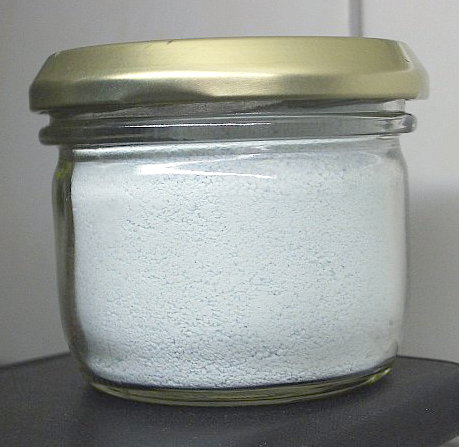
\includegraphics[width=\linewidth,height=4.2cm,keepaspectratio]{images/book1/cuso4-anhydrous.jpg}

{\small Sulfato de cobre anhidro: un polvo blanco. Foto: W.~Oelen,
CC BY-SA 3.0.}
\end{minipage}\hfill
\begin{minipage}[b]{0.48\linewidth}\centering
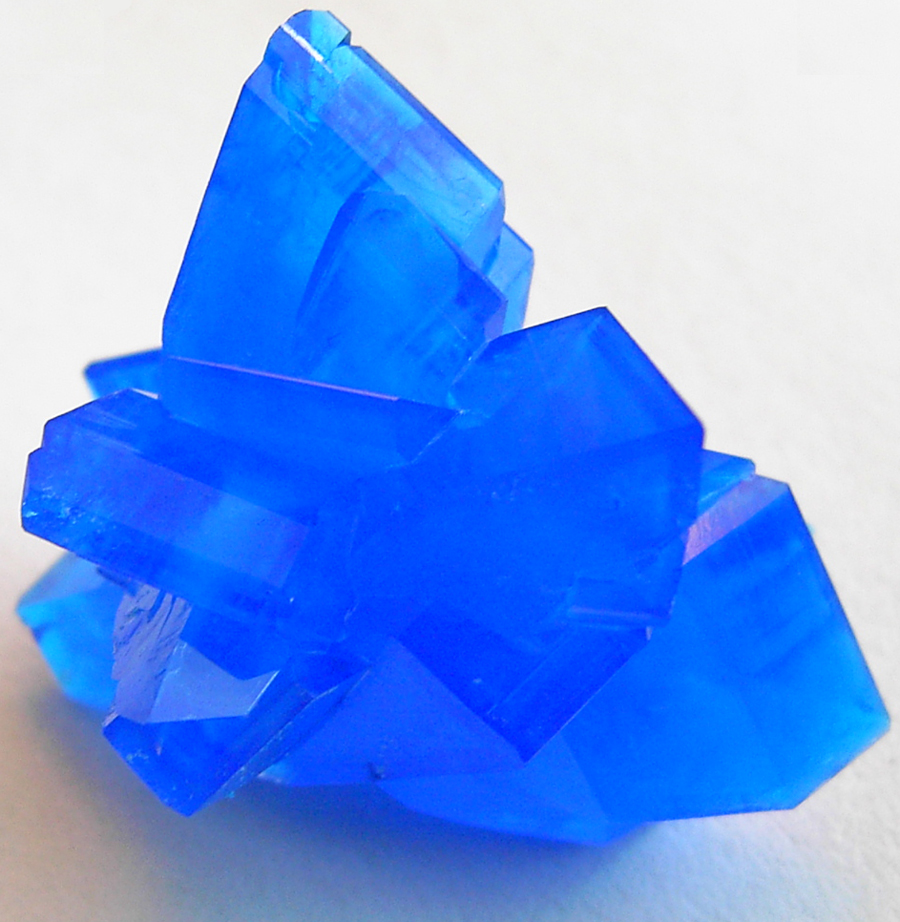
\includegraphics[width=\linewidth,height=4.2cm,keepaspectratio]{images/book1/cuso4-hydrated.jpg}

{\small Con agua se vuelve azul; estos cristales contienen agua. Foto:
Stephanb, CC BY-SA 3.0.}
\end{minipage}
\end{omfigure}

\begin{safety}{\ghs[0.82cm]{GHS05}\ghs[0.82cm]{GHS07}\ghs[0.82cm]{GHS09}}
% ledger: ghs:CuSO4
Sulfato de cobre: nocivo en caso de ingestión e irritante para la piel
(GHS07); puede causar lesiones oculares graves (GHS05); muy tóxico para
los organismos acuáticos, con efectos duraderos (GHS09). Gafas y
guantes; los residuos se recogen y nunca se tiran por el fregadero.
\end{safety}

\begin{proposition}[El oxígeno reaviva una astilla incandescente]\label{prop:g7:identifying-substances:splint}
Se enciende una astilla de madera y luego se sopla para apagarla, de
modo que solo quede una brasa roja. Introducida en un tubo de ensayo con
oxígeno, la astilla incandescente vuelve a \omterm{def:g4:what-a-fire-needs:burning}{arder} con llama.
\end{proposition}

\begin{proposition}[El hidrógeno arde con una pequeña detonación]\label{prop:g7:identifying-substances:pop}
Una astilla encendida acercada a la boca de un tubo de ensayo pequeño
con hidrógeno produce un ``pop'' breve y agudo: el hidrógeno \omterm{def:g4:what-a-fire-needs:burning}{arde} de
golpe con el oxígeno del \omterm{def:g4:air-a-mixture-of-gases:air}{aire}.
\end{proposition}

\begin{omfigure}
\begin{tikzpicture}[font=\small, scale=1.25]
  % splint test for oxygen
  \pic[transform shape] at (0,0) {testtube={0}{white}};
  \draw[brown!60!black, line width=2pt] (0.15,1.6) -- (1.4,3.6);
  \fill[orange!85] (0.15,1.6) circle (0.07);
  \fill[orange!80] (0.12,1.62) .. controls (0.0,1.9) and (0.08,2.1) .. (0.1,2.3)
    .. controls (0.2,2.05) and (0.3,1.85) .. (0.2,1.62);
  \node[anchor=north, align=center] at (0,-0.15) {oxígeno:\\ la astilla incandescente\\ vuelve a arder};
  % pop test for hydrogen
  \begin{scope}[xshift=4cm]
    \pic[transform shape, rotate=180] at (0,3.1) {testtube={0}{white}};
    \draw[brown!60!black, line width=2pt] (0.05,-0.05) -- (1.3,-0.9);
    \fill[orange!85] (0.05,-0.02) .. controls (-0.05,0.08) and (0.0,0.15) .. (0.02,0.22)
      .. controls (0.08,0.15) and (0.15,0.08) .. (0.1,-0.02);
    \node[font=\small\itshape] at (-0.9,0.15) {¡pop!};
    \node[anchor=north, align=center] at (0,-1.0) {hidrógeno:\\ un pop agudo\\ en la boca};
  \end{scope}
\end{tikzpicture}

{\small A la izquierda, una astilla incandescente vuelve a \omterm{def:g4:what-a-fire-needs:burning}{arder} en
oxígeno. A la derecha, una astilla encendida en la boca de un tubo de
hidrógeno boca abajo produce un pop agudo (el hidrógeno es más ligero
que el \omterm{def:g4:air-a-mixture-of-gases:air}{aire}, por eso el tubo se sostiene con la boca hacia abajo).}
\end{omfigure}

\begin{safety}{\ghs[0.82cm]{GHS02}\ghs[0.82cm]{GHS04}}
% ledger: ghs:H2
Hidrógeno: gas extremadamente inflamable (GHS02), almacenado a presión
en botellas (GHS04). El ensayo del pop se hace solo con unos pocos
mililitros, y lo hace el profesor.
\end{safety}

\section{La cromatografía en papel}

\begin{definition}[Cromatografía en papel y cromatograma]\label{def:g7:identifying-substances:chromatography}
La \emph{cromatografía en papel}\index{cromatografia en papel@cromatografía en papel} separa los
colorantes de una \omterm{def:g6:pure-substances-and-mixtures:mixture}{mezcla}. Se pone una pequeña mancha de la \omterm{def:g6:pure-substances-and-mixtures:mixture}{mezcla} sobre
una línea trazada cerca de la parte de abajo de una tira de papel; el
extremo inferior de la tira se sumerge en un \omterm{def:g6:solutions-and-solubility:solute}{disolvente}, que sube
despacio por el papel y arrastra cada colorante, unos más deprisa que
otros. Cuando el \omterm{def:g6:solutions-and-solubility:solute}{disolvente} ha subido casi hasta arriba, se saca la
tira y se seca: es el
\emph{cromatograma}\index{cromatograma}.
\end{definition}

\begin{omfigure}
\begin{tikzpicture}[font=\small, scale=1.3]
  % the strip in a beaker of solvent
  \pic[transform shape] at (0,0) {beaker={0.12}{omWater!80}};
  \fill[white] (-0.42,0.06) rectangle (0.42,2.2);
  \fill[omWater!80] (-0.42,0.06) rectangle (0.42,0.24);
  \draw[omGlass, line width=0.6pt] (-0.42,0.06) rectangle (0.42,2.2);
  \draw[black!60, line width=0.4pt] (-0.42,0.42) -- (0.42,0.42);
  \fill[black!80] (0,0.42) circle (0.07);
  \shade[ball color=black!20] (0,2.27) circle (0.08);
  \draw[black!50, line width=1.2pt] (-1.1,2.27) -- (1.1,2.27);
  \node[anchor=north, align=center] at (0,-0.15) {al principio};
  \draw[<-, omProp, thick] (0.1,0.5) -- (1.3,0.8) node[right, text=black]
    {mancha de tinta en la línea};
  \draw[<-, omProp, thick] (1.0,2.27) -- (1.3,2.5) node[right, text=black]
    {varilla que sujeta el papel};
  \draw[<-, omProp, thick] (0.75,0.15) -- (1.3,0.25) node[right, text=black]
    {disolvente, bajo la línea};
  % the chromatogram
  \begin{scope}[xshift=6.2cm]
    \pic[transform shape] at (0,0) {tlcplate};
    \draw[black!50, dashed] (-0.7,2.7) -- (0.7,2.7);
    \fill[blue!70] (0,1.0) ellipse (0.13 and 0.09);
    \fill[red!70] (0,1.7) ellipse (0.13 and 0.09);
    \fill[yellow!80!orange] (0,2.35) ellipse (0.13 and 0.09);
    \node[anchor=north, align=center] at (0,-0.15) {el cromatograma};
    \draw[<-, omProp, thick] (0.75,2.7) -- (1.3,2.85) node[right, text=black]
      {frente del disolvente};
    \draw[<-, omProp, thick] (0.2,1.7) -- (1.3,1.7) node[right, text=black]
      {tres colorantes: una mezcla};
  \end{scope}
\end{tikzpicture}

{\small \omterm{def:g7:identifying-substances:chromatography}{Cromatografía en papel} de una tinta negra. El \omterm{def:g6:solutions-and-solubility:solute}{disolvente} sube por
el papel y separa la tinta en tres colorantes.}
\end{omfigure}

\begin{method}[Leer un cromatograma]\label{met:g7:identifying-substances:read}
\begin{enumerate}
  \item Contar las manchas que hay encima de cada punto de partida: una
        mancha, un colorante; dos manchas o más, una \omterm{def:g6:pure-substances-and-mixtures:mixture}{mezcla} de
        colorantes.
  \item Comparar alturas: en un mismo \omterm{def:g7:identifying-substances:chromatography}{cromatograma}, un colorante sube
        siempre hasta la misma altura. Una mancha a la misma altura que
        un colorante conocido es probablemente ese colorante.
  \item Trazar la línea con lápiz, nunca con tinta: el \omterm{def:g6:solutions-and-solubility:solute}{disolvente}
        también separaría la tinta.
\end{enumerate}
\end{method}

\begin{example}[Los colorantes de los caramelos]\label{ex:g7:identifying-substances:sweets}
Se raspa la cobertura de colores de unos caramelos en un poco de agua y
se pone en manchas sobre una tira, junto a manchas de los colorantes
alimentarios autorizados en las golosinas. El \omterm{def:g7:identifying-substances:chromatography}{cromatograma} muestra que
la cobertura verde contiene un colorante amarillo y otro azul, ambos
entre los colorantes autorizados.
\end{example}


\section{Leer una tabla de ensayos}

\begin{proposition}[Una tabla de ensayos característicos]\label{prop:g7:identifying-substances:bank}
Los químicos reúnen los ensayos que usan en una tabla, una tabla de
ensayos, que se lee de izquierda a derecha:
\begin{center}
\small
\begin{tabular}{llll}
\hline
especie buscada & \omterm{def:g7:identifying-substances:characteristic-test}{reactivo} o ensayo & resultado positivo & \\
\hline
dióxido de carbono & agua de cal & el agua de cal se enturbia & \\
agua & sulfato de cobre anhidro & de blanco pasa a azul & \\
oxígeno & astilla incandescente & la astilla vuelve a \omterm{def:g4:what-a-fire-needs:burning}{arder} & \\
hidrógeno & astilla encendida & un pop agudo & \\
colorantes de una \omterm{def:g6:pure-substances-and-mixtures:mixture}{mezcla} & \omterm{def:g7:identifying-substances:chromatography}{cromatografía en papel} & una mancha por colorante & \\
\hline
\end{tabular}
\end{center}
\end{proposition}

\begin{remark}[Lo que un ensayo no dice]\label{rem:g7:identifying-substances:limits}
Un ensayo positivo demuestra que la especie está presente, no que esté
sola: un líquido que vuelve azul el sulfato de cobre contiene agua, pero
puede ser agua salada o zumo de naranja. Un ensayo negativo solo dice
que la especie no está, o que está en una cantidad demasiado pequeña
para notarse.
\end{remark}

\begin{omfigure}
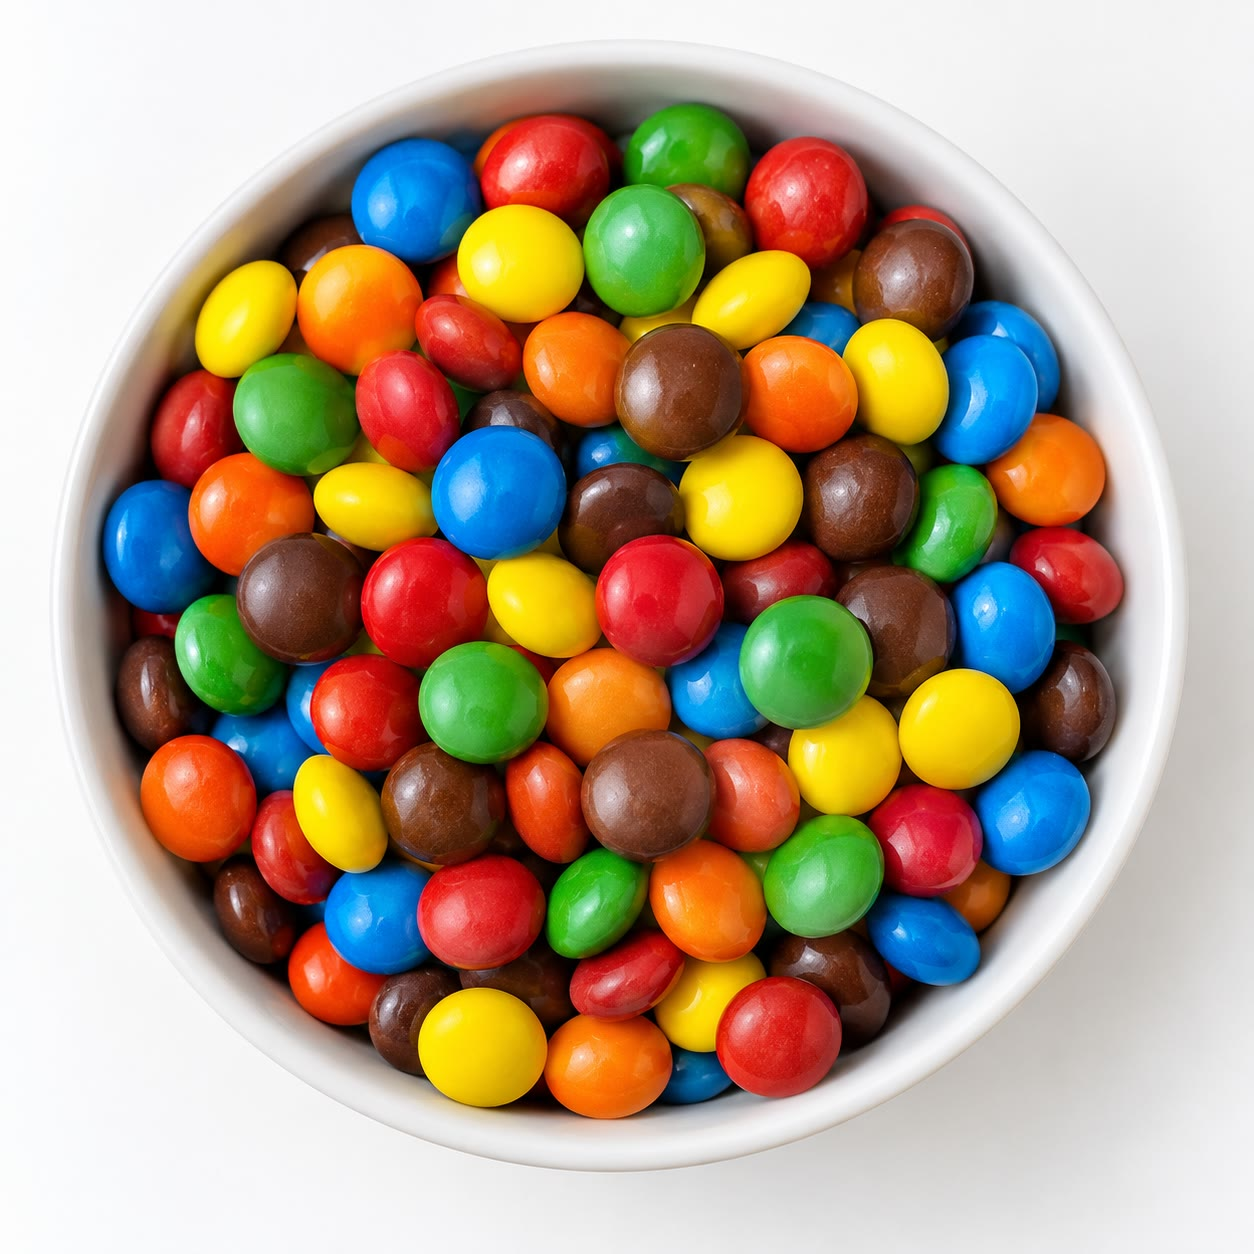
\includegraphics[width=0.32\linewidth]{images/book1/ai/g7-sweets.jpg}

{\small Caramelos con cobertura de azúcar: sus colores son \omterm{def:g6:pure-substances-and-mixtures:mixture}{mezclas} de
colorantes que la cromatografía puede separar.}
\end{omfigure}

\begin{omfigure}
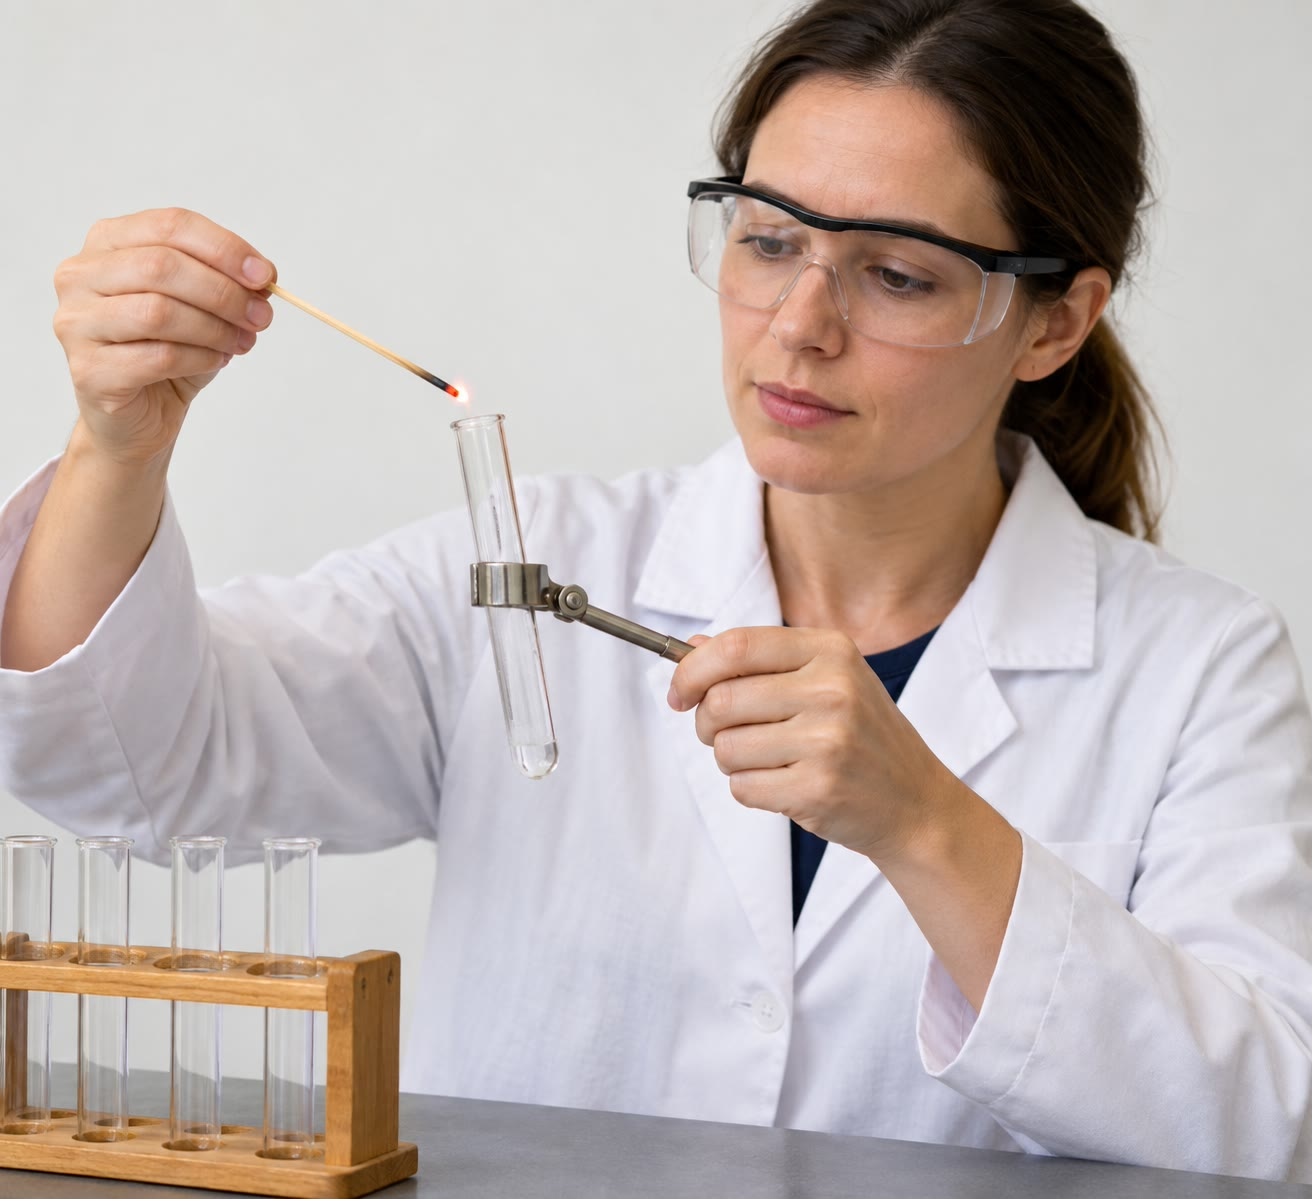
\includegraphics[width=0.36\linewidth]{images/book1/ai/g7-splint-teacher.jpg}

{\small Una profesora ensaya un gas con una astilla incandescente.}
\end{omfigure}

\section{Ejercicios}

\begin{exercise}[$\star$]\label{exo:g7:identifying-substances:1}
¿Qué ensayo identifica el dióxido de carbono? Describe su resultado
positivo.
\end{exercise}

\begin{exercise}[$\star$]\label{exo:g7:identifying-substances:2}
Un polvo blanco se vuelve azul cuando se le echa un líquido. ¿Qué
muestra esto sobre el líquido?
\end{exercise}

\begin{exercise}[$\star$]\label{exo:g7:identifying-substances:3}
Se introduce una astilla incandescente en un frasco de gas y vuelve a
\omterm{def:g4:what-a-fire-needs:burning}{arder} con llama. ¿Qué gas contiene el frasco?
\end{exercise}

\begin{exercise}[$\star$]\label{exo:g7:identifying-substances:4}
¿Por qué la línea de partida de un \omterm{def:g7:identifying-substances:chromatography}{cromatograma} en papel se traza con
lápiz y no con tinta?
\end{exercise}

\begin{exercise}[$\star\star$]\label{exo:g7:identifying-substances:5}
¿Por qué la línea de partida tiene que quedar por encima del nivel del
\omterm{def:g6:solutions-and-solubility:solute}{disolvente} en el vaso?
\end{exercise}

\begin{exercise}[$\star\star$]\label{exo:g7:identifying-substances:6}
El \omterm{def:g7:identifying-substances:chromatography}{cromatograma} de una tinta verde muestra dos manchas, una a la altura
de un colorante amarillo de referencia y otra a la altura de un
colorante azul de referencia. ¿Es la tinta verde una \omterm{def:g6:pure-substances-and-mixtures:pure-substance}{sustancia pura}? ¿De
qué está hecha?
\end{exercise}

\begin{exercise}[$\star\star$]\label{exo:g7:identifying-substances:7}
Con la tabla de ensayos, ¿qué ensayo usarías para mostrar que el gas
que desprende una reacción es hidrógeno? ¿Qué esperas ver?
\end{exercise}

\begin{exercise}[$\star\star$]\label{exo:g7:identifying-substances:8}
El \omterm{def:g4:air-a-mixture-of-gases:air}{aire} espirado enturbia el agua de cal mucho más deprisa que el \omterm{def:g4:air-a-mixture-of-gases:air}{aire}
fresco. ¿Qué nos dice esto sobre el \omterm{def:g4:air-a-mixture-of-gases:air}{aire} que espiramos?
\end{exercise}

\begin{exercise}[$\star\star$]\label{exo:g7:identifying-substances:9}
Un líquido transparente vuelve azul el sulfato de cobre anhidro. Sam
concluye: ``Es agua pura''. Explica por qué Sam se equivoca.
\end{exercise}

\begin{exercise}[$\star\star$]\label{exo:g7:identifying-substances:10}
Mira el \omterm{def:g7:identifying-substances:chromatography}{cromatograma} de la tinta negra de este capítulo. ¿Cuántos
colorantes contiene la tinta? ¿Cuál subió más alto?
\end{exercise}

\begin{exercise}[$\star\star\star$]\label{exo:g7:identifying-substances:11}
Tres frascos contienen oxígeno, hidrógeno y dióxido de carbono, pero han
perdido las etiquetas. Planifica, sobre el papel, los ensayos que
permitirían identificar cada frasco, en un orden que use el menor número
posible de ensayos.
\end{exercise}

\begin{exercise}[$\star\star\star$]\label{exo:g7:identifying-substances:12}
Un alumno ensaya un gas con agua de cal y no ve que pase nada. Da dos
explicaciones posibles, y el ensayo de control que ayudaría a decidir.
\end{exercise}

\section{Problema: La nota falsificada}

\begin{problem}[{Problema de fin de semana --- una nota escrita con
rotulador, tres rotuladores sospechosos, tres botellas de gas sin
etiqueta y una tabla de ensayos}]
\label{pb:g7:identifying-substances:1}
Se pide al laboratorio de un instituto que ayude a resolver dos pequeños
misterios. Primero, hay que relacionar una nota escrita con rotulador
negro con uno de tres rotuladores negros, 1, 2 y 3 (rot.~1, rot.~2 y
rot.~3 en la figura). Se toma una gota de tinta de la nota y de cada
rotulador y se ponen en manchas sobre la misma tira de papel, que
después se revela con agua. El \omterm{def:g7:identifying-substances:chromatography}{cromatograma} se muestra a continuación.
\begin{center}
\begin{tikzpicture}[font=\small, x=1cm, y=1cm]
  \fill[white] (0,0) rectangle (6,4);
  \draw[omGlass, line width=0.6pt] (0,0) rectangle (6,4);
  \draw[black!60] (0,0.5) -- (6,0.5);
  \draw[black!50, dashed] (0,3.6) -- (6,3.6);
  \foreach \x/\lab in {0.9/nota, 2.3/rot.~1, 3.7/rot.~2, 5.1/rot.~3}
    \node[anchor=north] at (\x,-0.05) {\lab};
  % note: three dyes
  \fill[blue!70] (0.9,1.2) ellipse (0.18 and 0.1);
  \fill[red!70] (0.9,2.2) ellipse (0.18 and 0.1);
  \fill[yellow!80!orange] (0.9,3.1) ellipse (0.18 and 0.1);
  % pen 1: two dyes
  \fill[blue!70] (2.3,1.2) ellipse (0.18 and 0.1);
  \fill[black!70] (2.3,2.7) ellipse (0.18 and 0.1);
  % pen 2: same three as the note
  \fill[blue!70] (3.7,1.2) ellipse (0.18 and 0.1);
  \fill[red!70] (3.7,2.2) ellipse (0.18 and 0.1);
  \fill[yellow!80!orange] (3.7,3.1) ellipse (0.18 and 0.1);
  % pen 3: three dyes, other heights
  \fill[violet!70] (5.1,0.9) ellipse (0.18 and 0.1);
  \fill[red!70] (5.1,1.8) ellipse (0.18 and 0.1);
  \fill[green!60!black] (5.1,2.6) ellipse (0.18 and 0.1);
  \node[anchor=west, font=\footnotesize] at (6.1,3.6) {frente del disolvente};
  \node[anchor=west, font=\footnotesize] at (6.1,0.5) {línea de partida};
\end{tikzpicture}
\end{center}

\medskip
\noindent\textbf{Parte I --- El \omterm{def:g7:identifying-substances:chromatography}{cromatograma}.}
\begin{enumerate}
  \item ¿Por qué se pusieron las cuatro tintas en la misma tira y se
        revelaron juntas?
  \item ¿La tinta de la nota es una \omterm{def:g6:pure-substances-and-mixtures:pure-substance}{sustancia pura} o una \omterm{def:g6:pure-substances-and-mixtures:mixture}{mezcla}?
        Explícalo.
  \item ¿Cuántos colorantes contiene la tinta del rotulador 1? ¿Pudo el
        rotulador 1 escribir la nota?
  \item El rotulador 3 también contiene tres colorantes. ¿Por qué no pudo
        escribir la nota?
  \item ¿Qué rotulador corresponde a la nota? Explícalo con las alturas
        de las manchas.
\end{enumerate}

\medskip
\noindent\textbf{Parte II --- Tres botellas de gas.}
El segundo misterio: tres pequeñas botellas, X, Y y Z, han perdido las
etiquetas; contienen oxígeno, hidrógeno y dióxido de carbono. Se recoge
un poco de gas de cada una en un tubo de ensayo. El gas X reaviva una
astilla incandescente. El gas Y produce un pop agudo con una astilla
encendida. El gas Z enturbia el agua de cal.
\begin{enumerate}[resume]
  \item Nombra el gas X.
  \item Nombra el gas Y.
  \item Nombra el gas Z.
  \item Antes de ensayar el gas Z, el alumno hace burbujear \omterm{def:g4:air-a-mixture-of-gases:air}{aire} normal
        a través de la misma agua de cal durante el mismo tiempo, y
        sigue transparente. ¿Cómo se llama este segundo ensayo, y qué
        añade a la conclusión?
\end{enumerate}

\medskip
\noindent\textbf{Parte III --- La tabla de ensayos.}
\begin{enumerate}[resume]
  \item Un líquido incoloro encontrado junto a la nota vuelve azul el
        sulfato de cobre anhidro. Escribe la línea de la tabla de
        ensayos utilizada y lo que muestra el resultado.
  \item ¿Demuestra este resultado que el líquido es agua pura?
        Explícalo.
  \item Concluye el primer misterio: ¿cuántos colorantes contiene la
        tinta de la nota, y qué rotulador la escribió?
\end{enumerate}
\end{problem}
